% \documentclass[aps,prl,twocolumn,superscriptaddress]{revtex4-1}
\documentclass[twocolumn]{revtex4-2}

\usepackage{graphicx}  
\usepackage{amssymb}   
\usepackage{verbatim}  
\usepackage{color}
\usepackage{amsmath}
\usepackage{booktabs}
\usepackage{caption}
\usepackage{subcaption}
\usepackage{epstopdf}
\usepackage{hyperref}
\hypersetup{
    colorlinks,
    citecolor=black,
    filecolor=black,
    linkcolor=black,
    urlcolor=black
}
\usepackage{tocloft}


% \addtolength{\cftsecnumwidth}{20pt}
% \addtolength{\cftsubsecnumwidth}{20pt}
% \addtolength{\cftfignumwidth}{10pt}


\bibliographystyle{apsrev}



\textheight=9in
\textwidth=6.5in
\oddsidemargin=0cm
\evensidemargin=0cm


\begin{document}


\title{Creating a Basic Laser Projector}


\author{\textbf{Robert Strauss}} 
\affiliation{Department of Physics,\\ 13 June 2025}



\begin{abstract}

We engineered and built a laser projector  capable of projecting a simple binary-value monochrome image on a nearby screen by rapidly modulating a laser diode reflected off quickly moving mirrors scanning a path through the image region. One mirror is a dodecagon with reflective surfaces, spun to about 3000 RPM. The angle of the beam continuously changes as the reflecting face rotates, then discontinuously jumps back to where it began as a corner of the polygon crosses the beam. The second mirror is a flat circle spun at an axis askew from its normal, at slightly slower speeds, about 2000 RPM. A beam reflected off this mirror traces a cone, projecting an ellipse. At sufficiently steep angles this ellipse is significantly longer in one direction, giving the second axis of control of the beam's position. Timing sensors detect the phase and rate of rotation of each mirror, feeding signals into a microcontroller which modulates the power to the laser diode in the 100 kHz regime. As the laser rasters across a 2d region where an image can be projected, the laser illuminates only specific points to create an image. Due to the high speed of the process, human persistence of vision allows observers to see a fixed image where only a quickly moving point of light exists.
 
\end{abstract}

\maketitle    
\vspace*{0em}
\noindent\textbf{\large CONTENTS}\par
\vspace*{-2.5em}
\tableofcontents
\vspace*{3em}
\noindent\textbf{\large LIST OF FIGURES}\par
\vspace*{-2.5em}
\listoffigures
% \clearpage


\section{Introduction}

\subsection{Similar Work}

Laser projectors such as this have been created before by many independent creators. We were particularly inspried by "Ben Makes Everything" \cite{ben}, who documented his process in video format online. Ben's setup uses a very small lightweight dodecagon mirror stripped from a laser printer spinning at high speed to scan the laser beam horizontally at very high frequency, and a high-speed galvanometer mirror to angle the scanning line vertically. Together this allows the rastered rendering of an image by illuminating or not illuminating the laser as it scans through each pixel, akin to the working of a cathode ray tube television set. Human persistence of vision allows for the quickly moving illuminated dot to appear as a continuous image.

\subsection{Polygon Mirror}

The polygon mirror is an essential trick for this kind of raster-based (tracing each line all the way across) laser projecting, as opposed to vector-based imaging such as that in a vector monitor where only the path of the desired edges of the image are traced. The latter requires rapid changes in the motion of the mirrors, to trace a specific path. The polygon mirror technique avoids this by constantly spinning at a fixed rate. It doesn't have to stop and decelerate even to return to the beginning of the next line, since the edges result in the angle of incidence changing suddenly and discontinuously as they rotate into the beams path. The second dimension still requires a galvanometer arm since after the first reflection, the beam may be anywhere in a wide arc, so the second polygon would have to be very deep. Luckily the second axis can scan much more slowly than the first, by a factor of the horizontal resolution. The scan angle of a polygon mirror is 

\begin{equation}
    \Delta \theta = \frac{4 \pi}{N}
    \label{eq:scan}
\end{equation}

where $\Delta \theta$ is the arc length of the scan, and $N$ is the number of sides of the polygon. The factor $4\pi$ may be confusing: intuitively we expect at most a prefactor of 2 on $\pi$, for the $2\pi$ radians spanning a circle. The resolution to this is, in short, reflections effectively double the angle of a beam as each change in the angle of the mirror changes the angle of incidence and thus also the angle of reflection, doubling the change in the angle of the reflected beam relative to the incident beam. This means a 12-sided  mirror has a scan angle of $60^{\circ}$, more than enough arc length to work with.

\subsection{Constraints}
The main physical constraint of the project is moving and modulating the beam fast to appear as a continuous image to the human eye, drawing a whole image within the timescale of human persistence of vision. According to Wyant College of Optical Sciences \cite{wyant} this is about 1/15th of a second. This means the second axis mirror needs to return to its position, completing a full image, at 15Hz minimum. The first mirror would then have to be a factor of the vertical resolution faster (100 vertical pixels = 100 cycles of first mirror for one cycle of the seccond). The polygon mirror presents a clear advantage in not having to rapidly accelerate and decelerate mirrors in the kilohertz regime. However even the 10s of Hertz required for the second mirror is still a challenge.

Without the exact parts and tooling available to Ben Makes Everyting, his construction could not simply be repeated like a cookbook; and we were under tighter budget and time constraints than this creator. The polygon mirror we purchased was much larger and bulkier than that used by Ben, this being the only available 12-sided mirror we could find within our budget and time limit. Other fewer-sided mirrors were available, but having fewer sides dramatically increases the scan angle, requiring lower resolution and faster spinning to still paint an entire image within the human persistence of vision timescale. (See eq.~\ref{eq:scan}).

For the second axis, the ideal solution of a several-inch deep polygon mirror (to catch the beam anywhere in its now wide arc), is not a part that is made or sold anywhere. The second best option is a galvanometer arm. However due to decent galvanometers from trustworthy sources costing at least 150 USD, this was outside of the budget for this project, so we came up with our own creative solution, detailed in section~\ref{2d}.



\section{Methods}

\subsection{One Dimension}

We begin by getting just a one-dimensional 'image' projector working (able to draw an arbitrary "Morse-code" like pattern on the screen).

Beyond just getting a polygon mirror spinning and reflecting a laser, we must be able to know exactly where it is reflecting this laser to modulate the laser in time to create a still image. The solution we came up with was using a secondary laser and photoresistor to detect when the laser scans by. This and the projection laser have to be precisely aligned and conveniently adjustable, so we modeled and 3d-printed laser-holding structures adjustable in height, yaw, and pitch. The apparatus is shown in Figure~\ref{fig:scan-sensor}. The laser passing across the photoresistor makes it more conductive, decreasing the voltage across it if wired in series with another resistor. The signal appears as brief spikes of low voltage, shown in Figure~\ref{fig:spike-signal}. A piece of cardboard with vertical slits for the laser and photoresistor was placed in front of the two in order to make the spieks even narrower, occurring only on the precise overlap of two narrow slits rather than gradually growing as the circular beam profile overlaps the photoresistor more. This made our triggering more precise, improving horizontal resolution and image stability. From this spike signal we can compute the rate of scan of the laser, and combining this with the time since the last scan we can compute the exact phase of the laser's cycle.




\begin{figure}
    \centering
    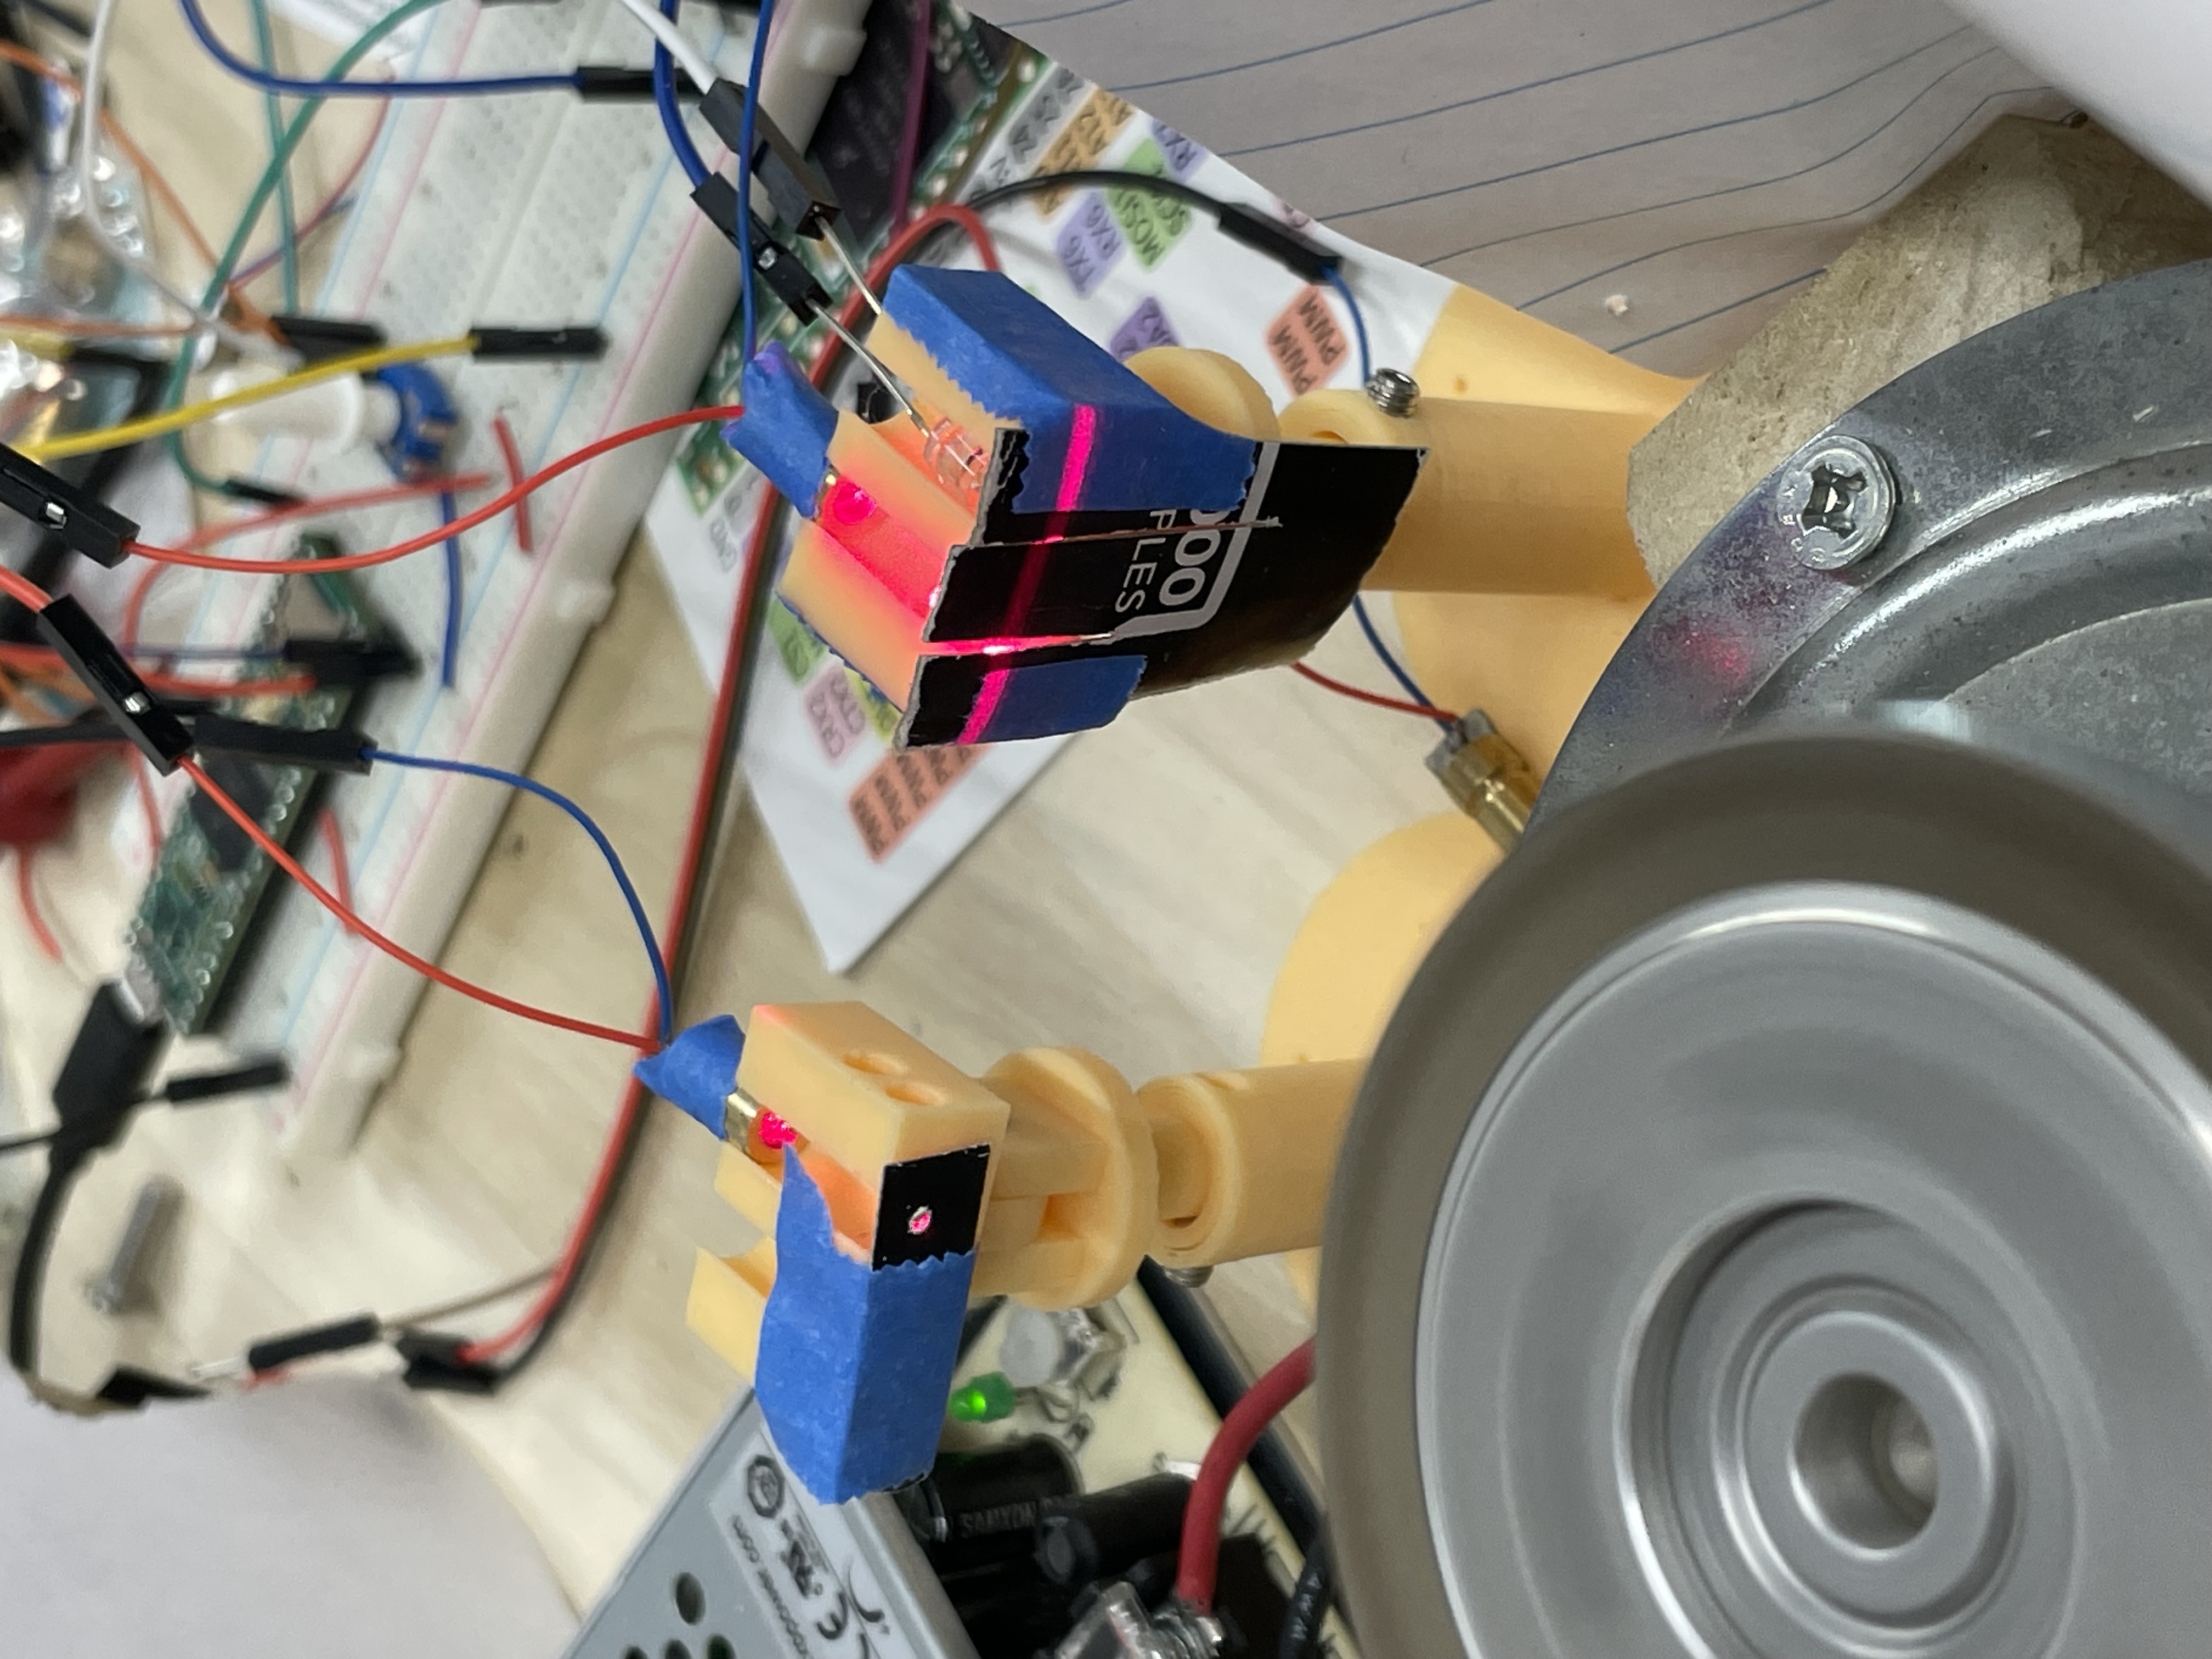
\includegraphics[angle=270,width=0.95\linewidth]{scan-sensor.jpeg}
    \caption[Scan Sensor]{Scan sensor detects each side of the polygon mirror rotating by by reflecting a laser off of it into a photoresistor, creating a spike signal used to calculate the rate of rotation and current angle of the mirror (based off the rate and time since the last spike). The spike signal produced by this device is shown in Figure~\ref{fig:spike-signal}.}
    \label{fig:scan-sensor}
\end{figure}



\begin{figure}
    \centering
    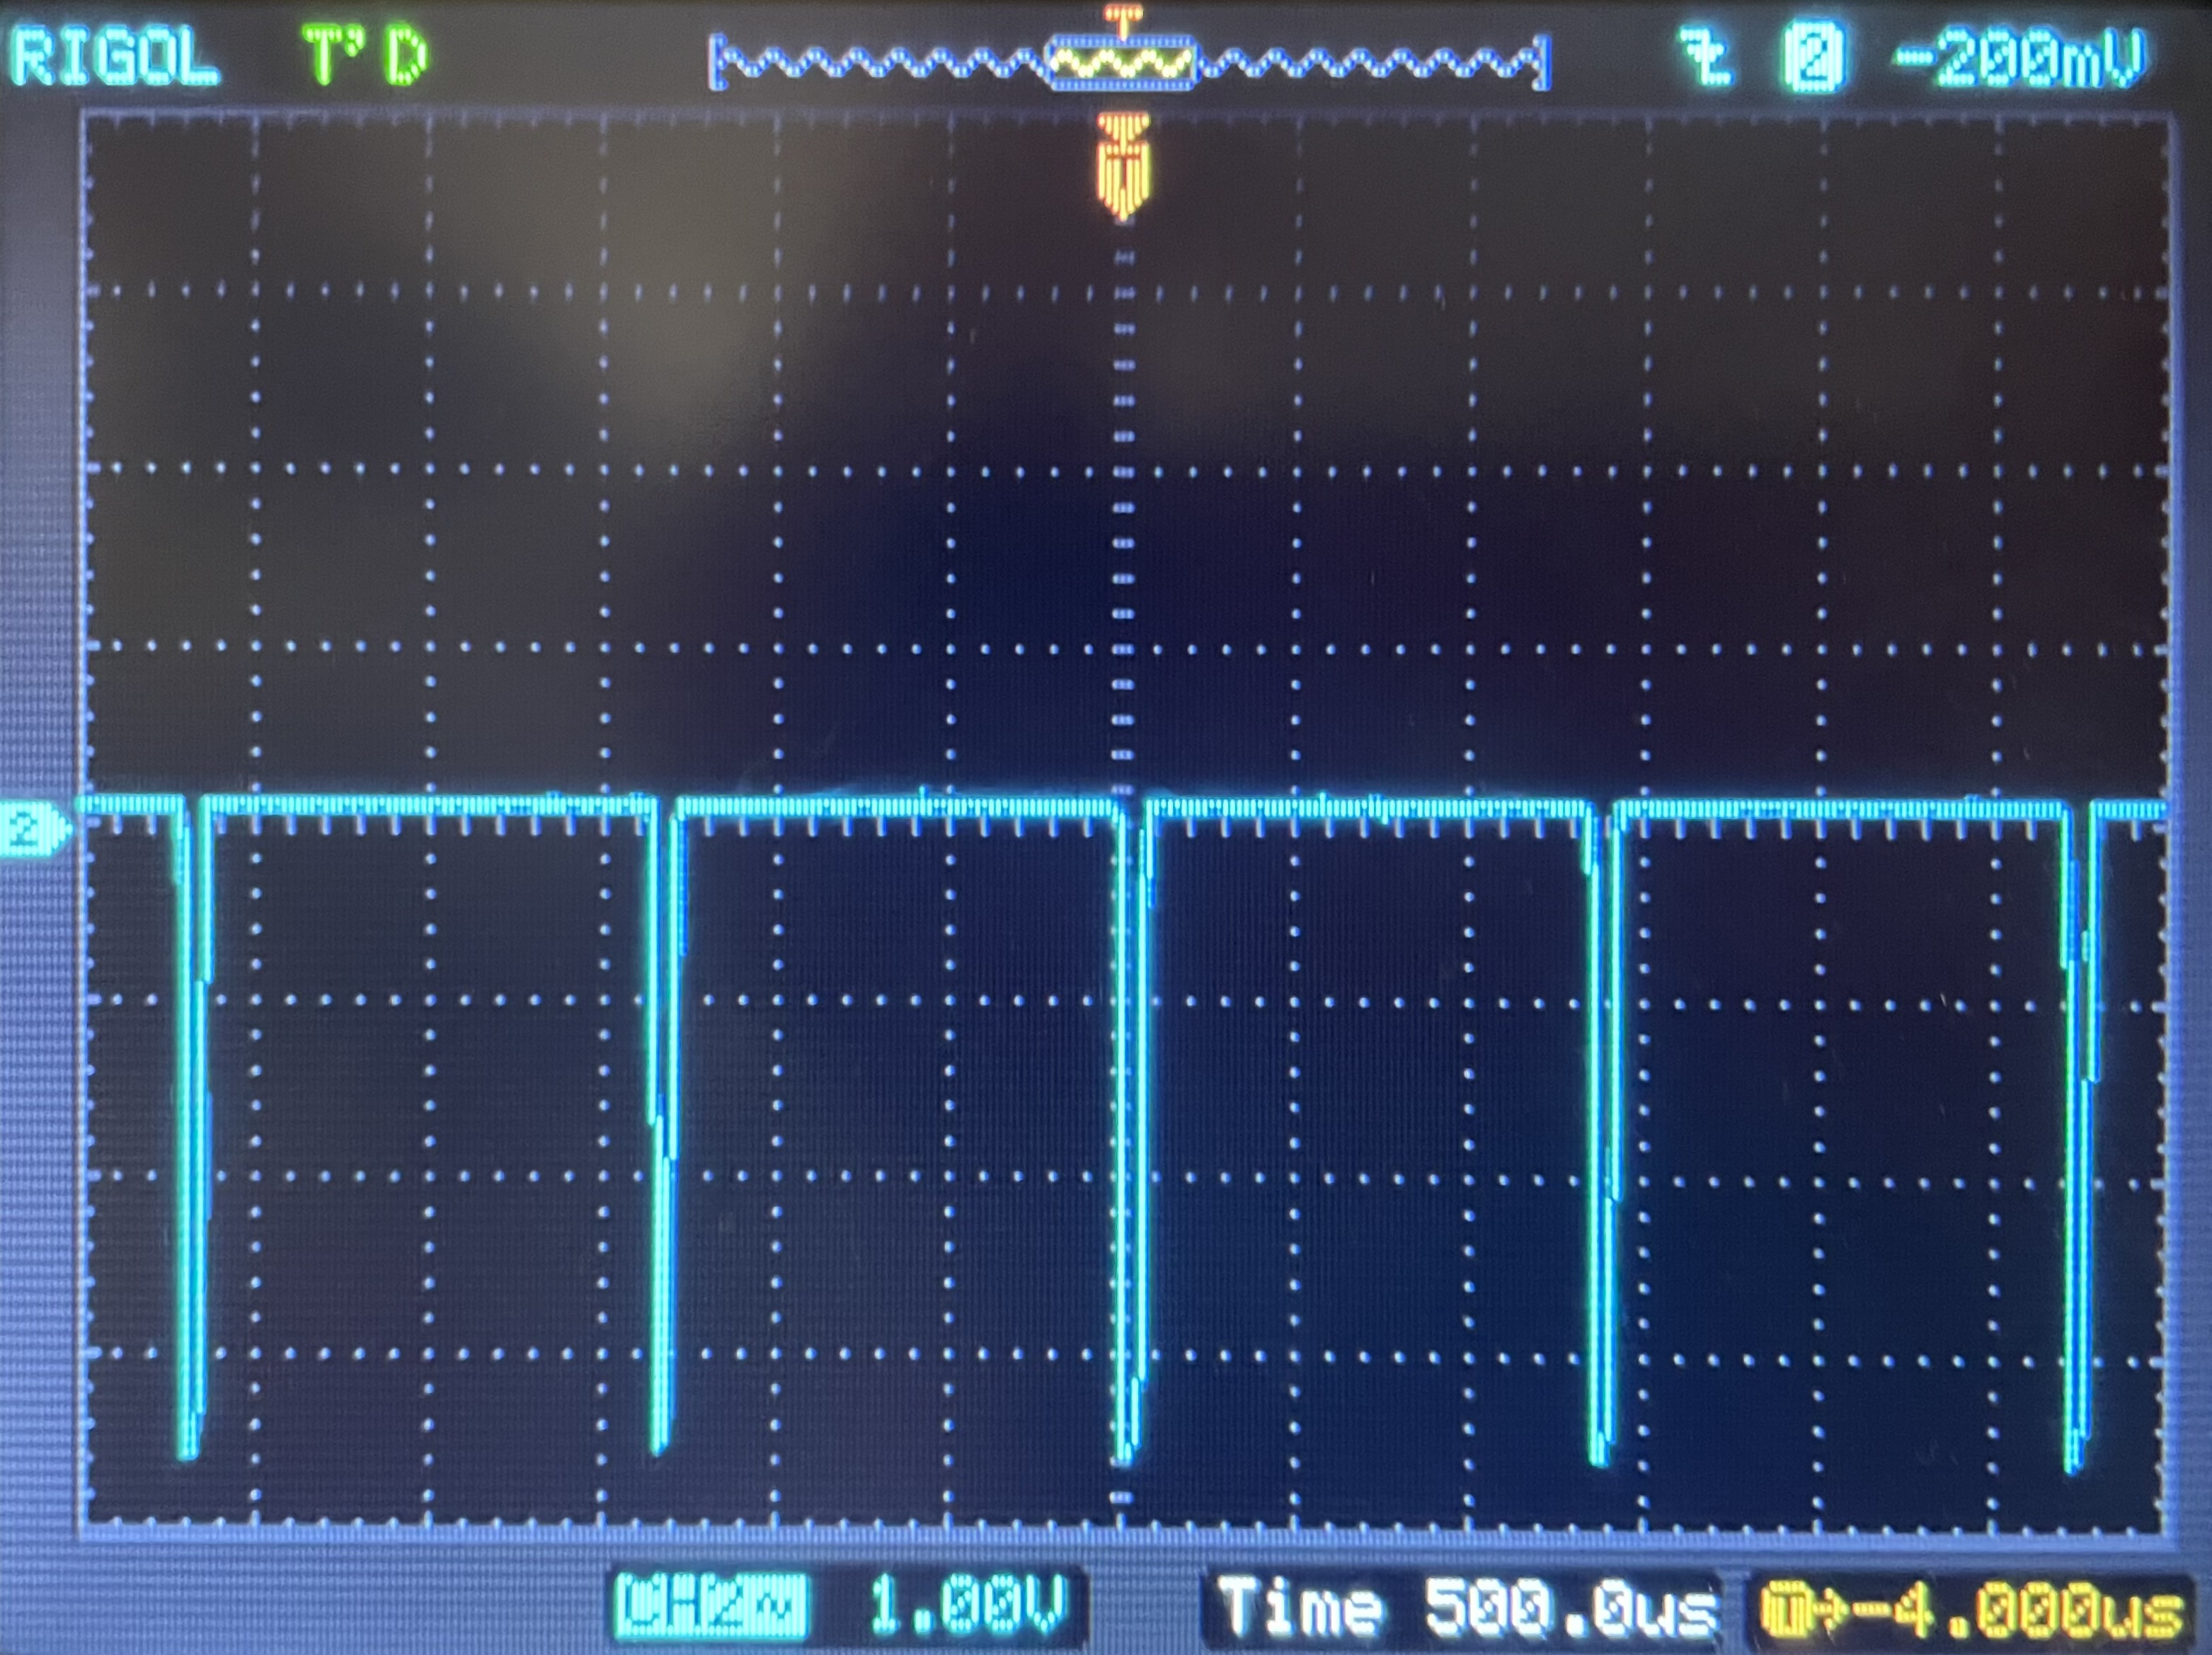
\includegraphics[width=0.95\linewidth]{spike-signal.jpeg}
    \caption[Scan Timing (Spike) Signal]{Spike signal produced by laser rapidly sweeping across photoresistor as polygon mirror rotates. This signal is fed into the microcontroller to calculate the rate of rotation of the mirror and position of a beam reflected off it given the calculated rate time since the last spike, letting our program know where on the screen the laser is currently pointed and determine whether to illuminate this point or not based on the desired image.}
    \label{fig:spike-signal}
\end{figure}

There is an unknown phase difference between the scan detector laser and the projector laser based on  the different spots on the polygon these reflect, and the scan sensor measurement only gives a relative not absolute phase, since we don't know precisely where in the scan relative to the edge jump the photoresistor is placed. We solve the relative phase issue by adding a potentiometer (measured as an analog voltage by the microcontroller) with which the user can set an arbitrary phase offset, to place the image in the desired position. 



\begin{figure}
    \centering
    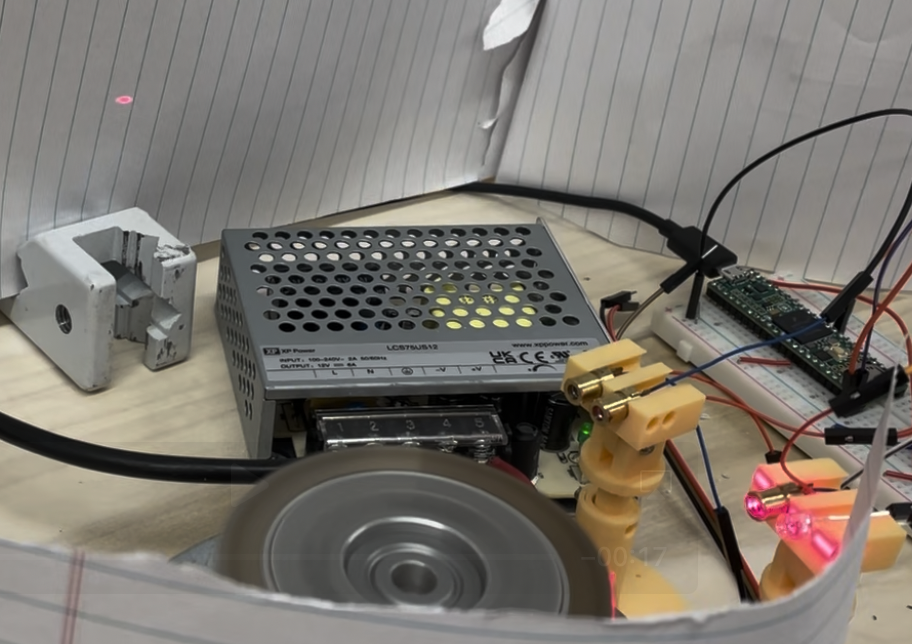
\includegraphics[width=0.95\linewidth]{still-dot.png}
    \caption[Still Dot]{Top left: small red dot (top left) is held fixed on page, despite reflecting off a rapidly spinning polygon mirror (bottom middle). When not precisely timed using the scan sensor, the beam traces a $60^{\circ}$ arc, and appears as a long line on the page. This demonstrates the success of the spike sensor (bottom right) and timing program (microcontroller middle right).}
    \label{fig:still-dot}
\end{figure}



Figure~\ref{fig:still-dot} shows the success of this setup: we can draw a still dot on the screen, despite the projecting laser reflecting off the rapidly rotating mirror. Although trivial, as a still laser could have instead been shown directly on the screen to produce the same effect, this is a demonstration we can in fact synchronize the timing of laser illumination reflected off quickly moving mirrors. Without modulating the laser, the result would be a long line draw across the page, as the beam scans through its $60^{\circ}$ arc. We can precisely time the modulation of the laser to produce the illusion of a single still dot. More complicated patterns were also tested, including alternating patterns to find the maximum horizontal resolution allowed by the precision of our triggering apparatus. We find the image appears stable and clear through time beyond 128 pixels across, beyond which we don't bother testing.


\subsection{Two Dimensions} \label{2d}

The second dimension makes things substantially more complicated, especially without the convenience of a high-speed galvanometer to quickly and linearly move the beam vertically. Hardly any other hardware can accomplish the same goal of rapidly (15Hz * vertical resolution $\approx$ 1 kHz for about 100 pixels) and precisely (arc / vertical resolution / 2 $\approx$ $0.2^{\circ}$ step) accelerating and decelerating a mirror, within the tight budget used here. Our solution takes inspiration from the breakthrough of the polygon mirror: avoiding the battle with inertia altogether. By spinning a mirror slightly off if its normal axis, the reflected beam traces a cone. The part we designed for this is shown in Figure~\ref{fig:tilt-mirror-profile}. Indeed, even with constant rotation a tilted mirror does require torque due to the principal axes not being parallel to the axis of rotation. So we counterbalance the mirror with bolts configured to position the center of mass in line with the axis of rotation and a principal axis parallel to the rotation. We developed software extending our CAD model to visualize the principal axes and center of mass in real time as the model is developed and refined, such that the holes for bolts can be placed correctly.

The spinning tilted mirror results in a circular projected beam path, which is suboptimal, since when combined with the horizontal scanning of the polygon mirror this would create regions traced twice by the projector but also regions traced only once, creating a bright middle region but dimmer and round edge regions. Taking inspiration from the way a sunset on the ocean creates a long narrow reflection, despite isotropic roughness of the ocean surface, we realized by making the angle of incidence of the laser onto the tilted mirror not head on but quite steep, the path becomes a very eccentric ellipse, which is closer to a purely flat vertical line scanning up and down. The geometry of the reflection from the polygon mirror makes it difficult to be maximally steep and maximally eccentric, the achieved ellipse traced is shown in Figure~\ref{fig:ellipse-trace}. Although a confusing coordinate system, the horizontal and elliptical scanning can be dealt with in software. 

\begin{figure}
    \centering
    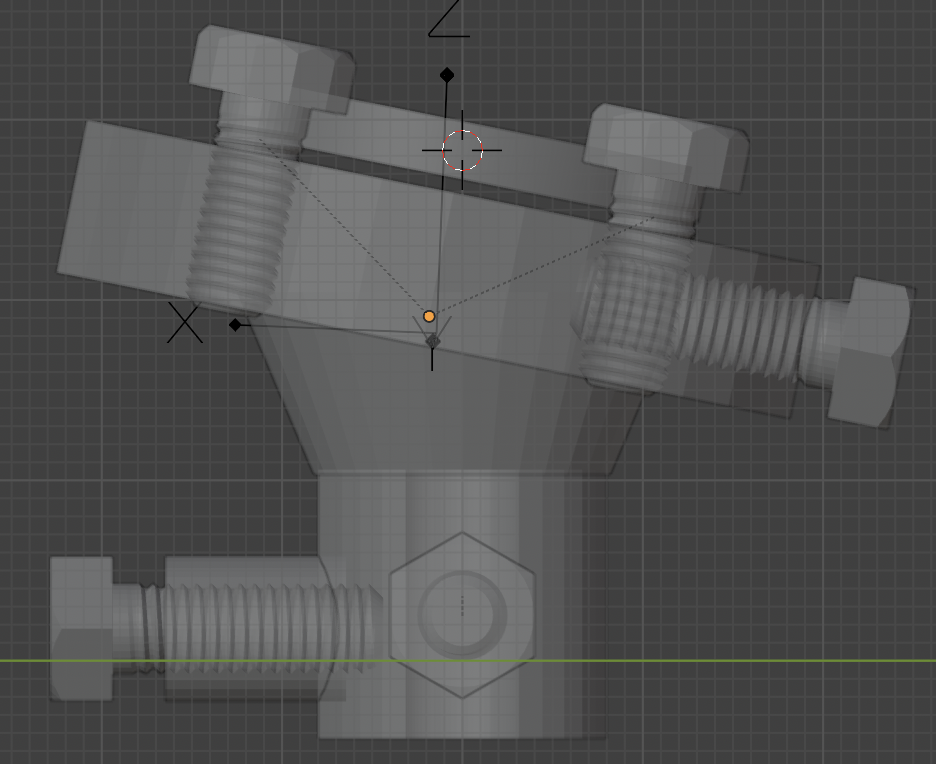
\includegraphics[width=0.95\linewidth]{tilt-mirror-profile.png}
    \caption[Tilted Mirror Mount Blueprint]{The design for a mirror-motor mount, rotating the tilted mirror on an axis not parallel with its normal vector. The mount to the motor is 3d printed, with extra holes for bolts included in order to balance the moment of inertia, placing the principal axis ("Z" arrow, also "X" and "Y" other principal axes) in line with the axis of rotation. A program was developed to compute the principal axes, allowing the correct geometry to be modeled and printed.}
    \label{fig:tilt-mirror-profile}
\end{figure}


\begin{figure}
    \centering
    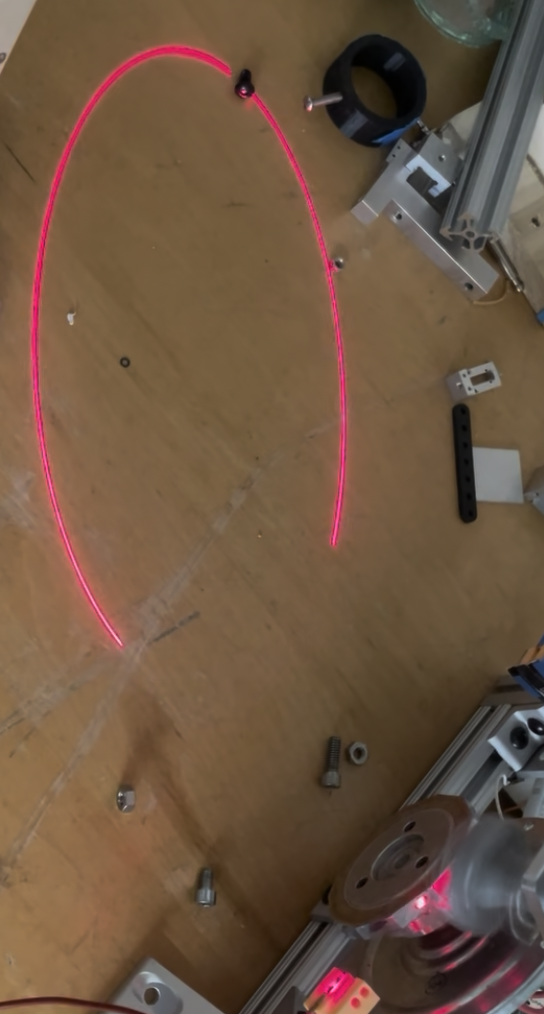
\includegraphics[width=0.95\linewidth]{ellipse-trace.png}
    \caption[Elliptical Path from Tilted Mirror]{The elliptical path traced by the conical arc of the beam reflected off the rotating tilted mirror. The ellipse can be made eccentric not only by elongating it with a more steep angle of projection, but also making it narrower by making the angle of incidence of the beam onto the mirror more steep. }
    \label{fig:ellipse-trace}
\end{figure}



Similar to the polygon scanner, we need to detect the rate and current phase of the mirror. A beam waving around ain an eccentric conical shape in 3d is not only much more difficult to place a photoresistor to detect, but also dangerous to eyesight. Instead, we use an inductor near the base of the mirror holder and attach a small magnet to one of the bolts protruding from this base, passing very close by the inductor and generating an EMF with every rotation. This design is pictured in Figure~\ref{fig:tilt-mirror-sensor}. The spike signal from this apparatus, simultaneously with the polygon mirror spike signal, are shown in Figure~\ref{fig:dual-spike-signals}. The polygon mirror is much more frequent, since this must draw some number of lines for each cycle of the tilted mirror. 


\begin{figure}
    \centering
    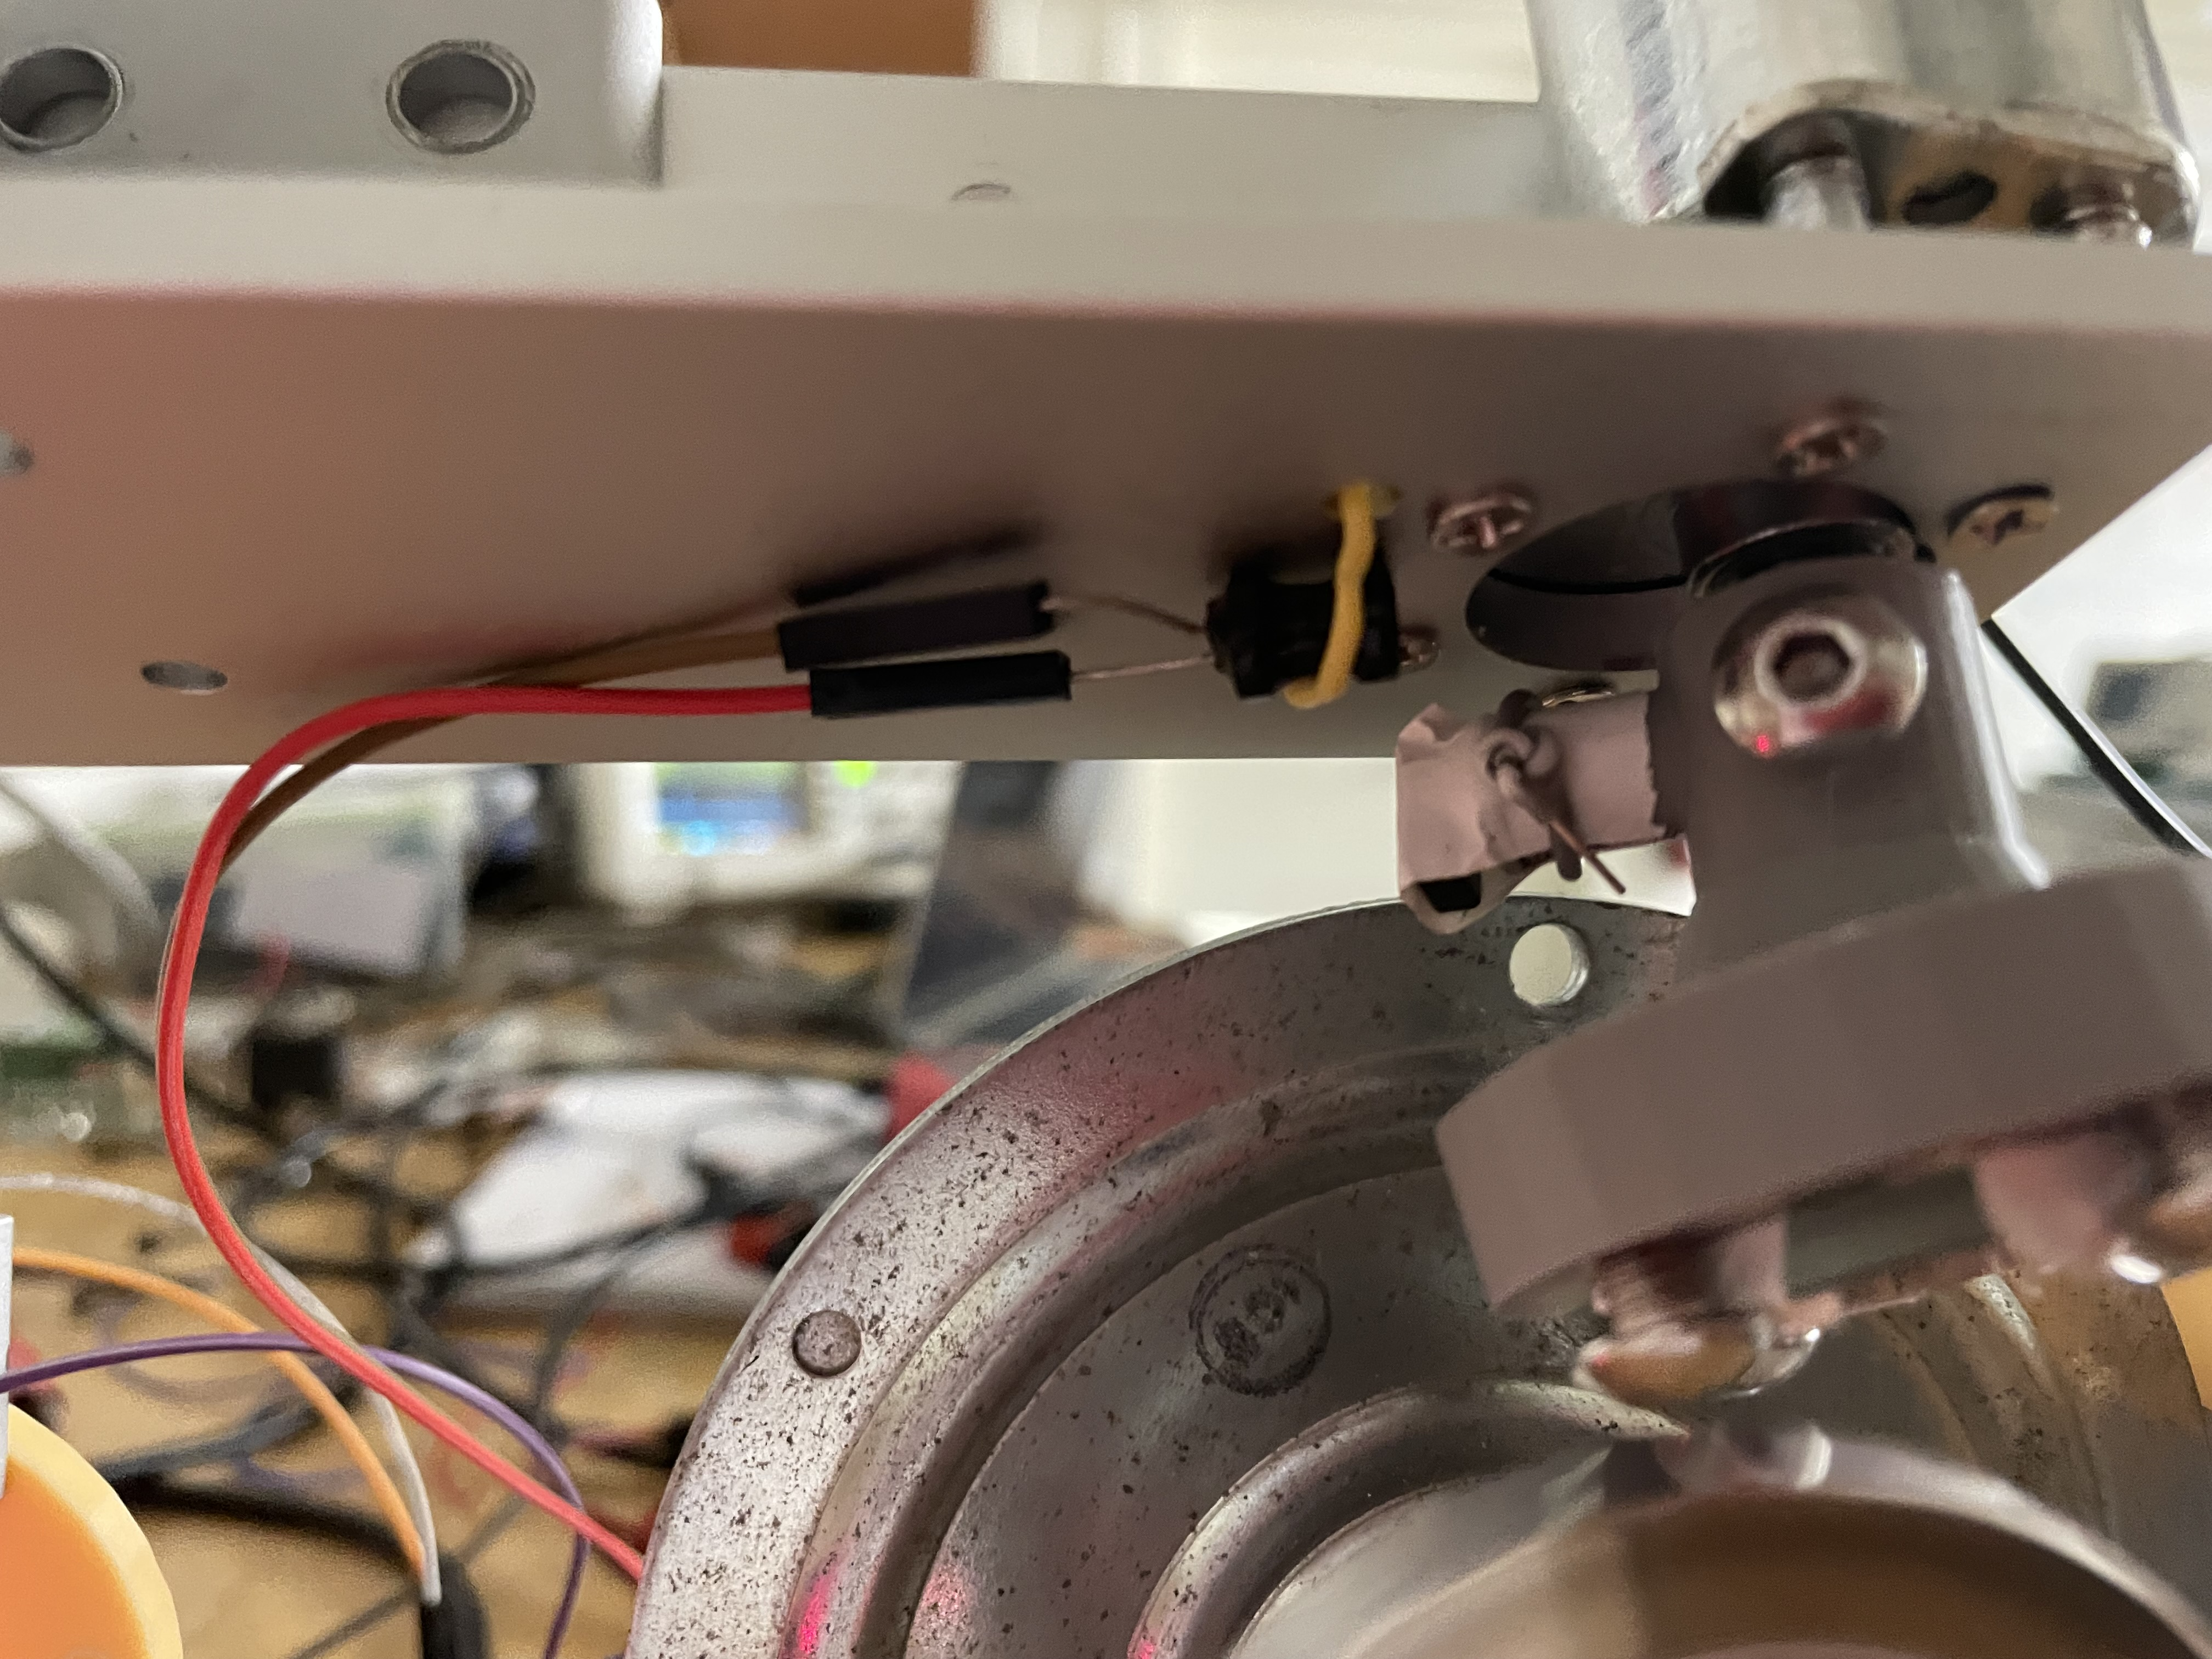
\includegraphics[width=0.95\linewidth]{tilt-mirror-sensor.jpeg}
    \caption[Tilted Mirror Rotation Sensor]{An inductor detects the changing magnetic field from a magnet attached to the mirror mount as it spins, creating a timing spike signal analogous to the laser scan sensor.}
    \label{fig:tilt-mirror-sensor}
\end{figure}



\begin{figure}
    \centering
    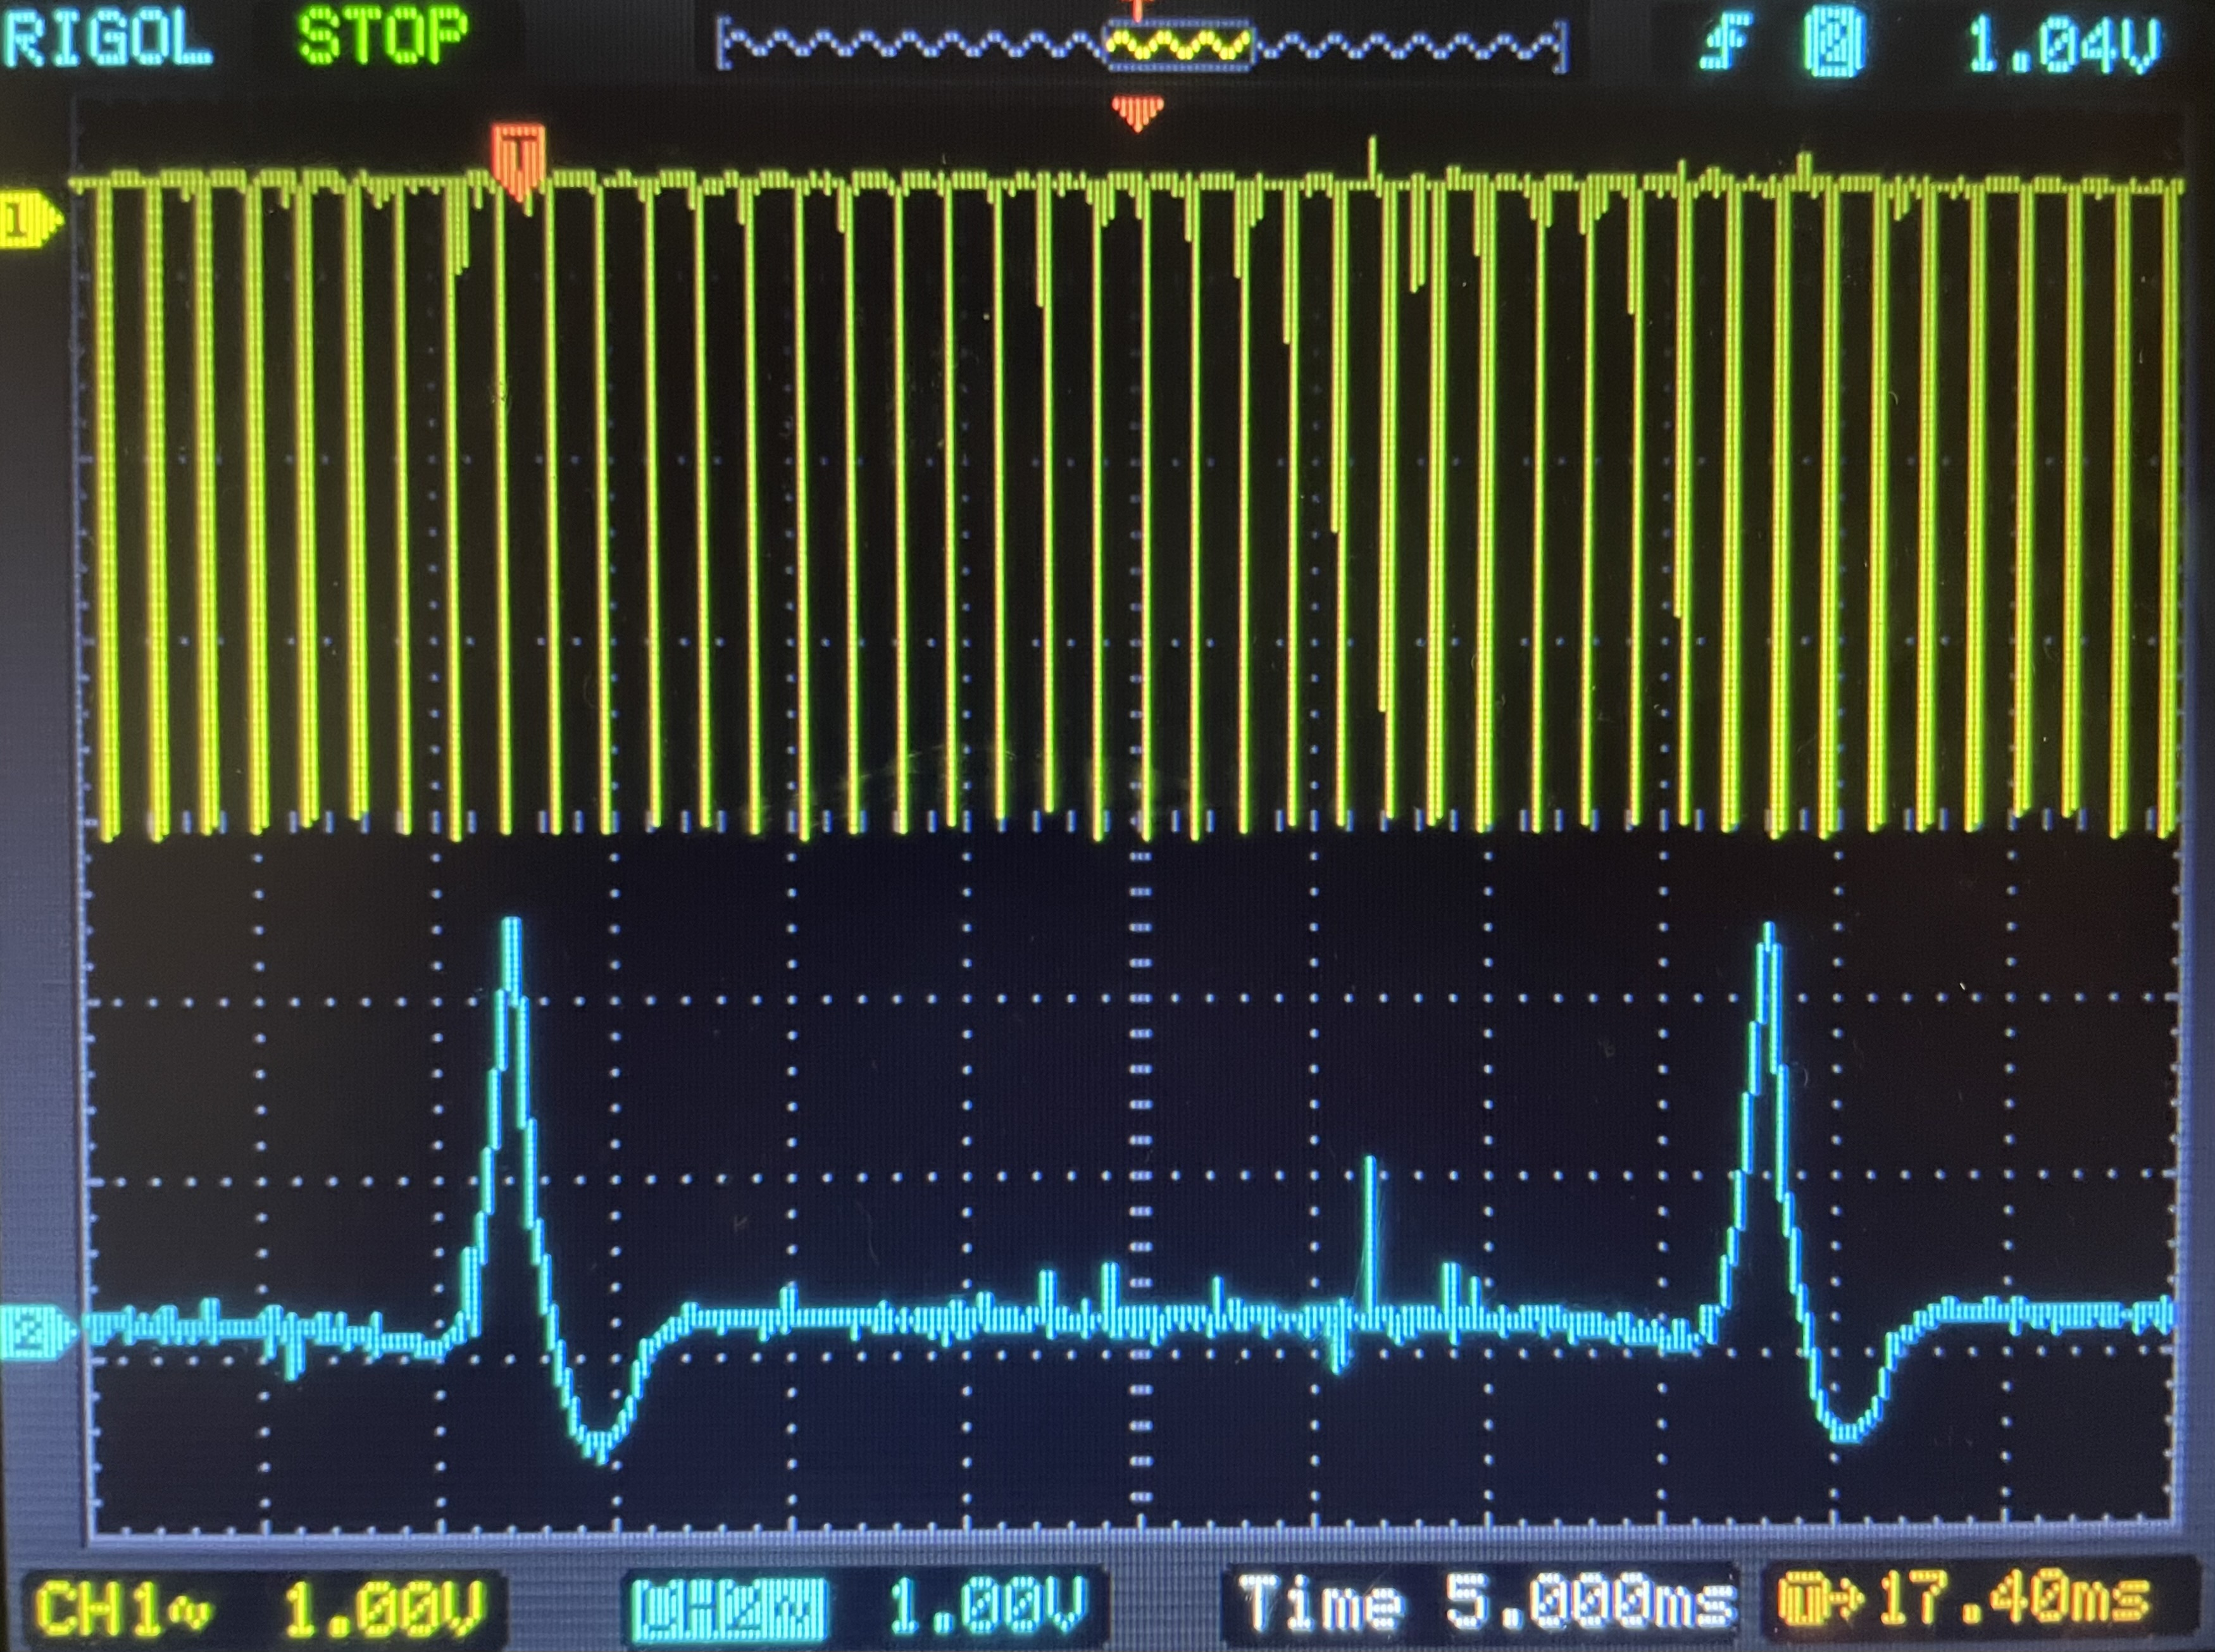
\includegraphics[width=0.95\linewidth]{dual-spike-signals.jpeg}
    \caption[Both Timing Signals]{The laser scan sensor (yellow) and tilted mirror (blue) timing signals. The yellow is much more frequent, since each spike corresponds to one horizontal line drawn, and there should be many of these for each vertical repetition drawing another frame. }
    \label{fig:dual-spike-signals}
\end{figure}


\begin{figure}
    \centering
    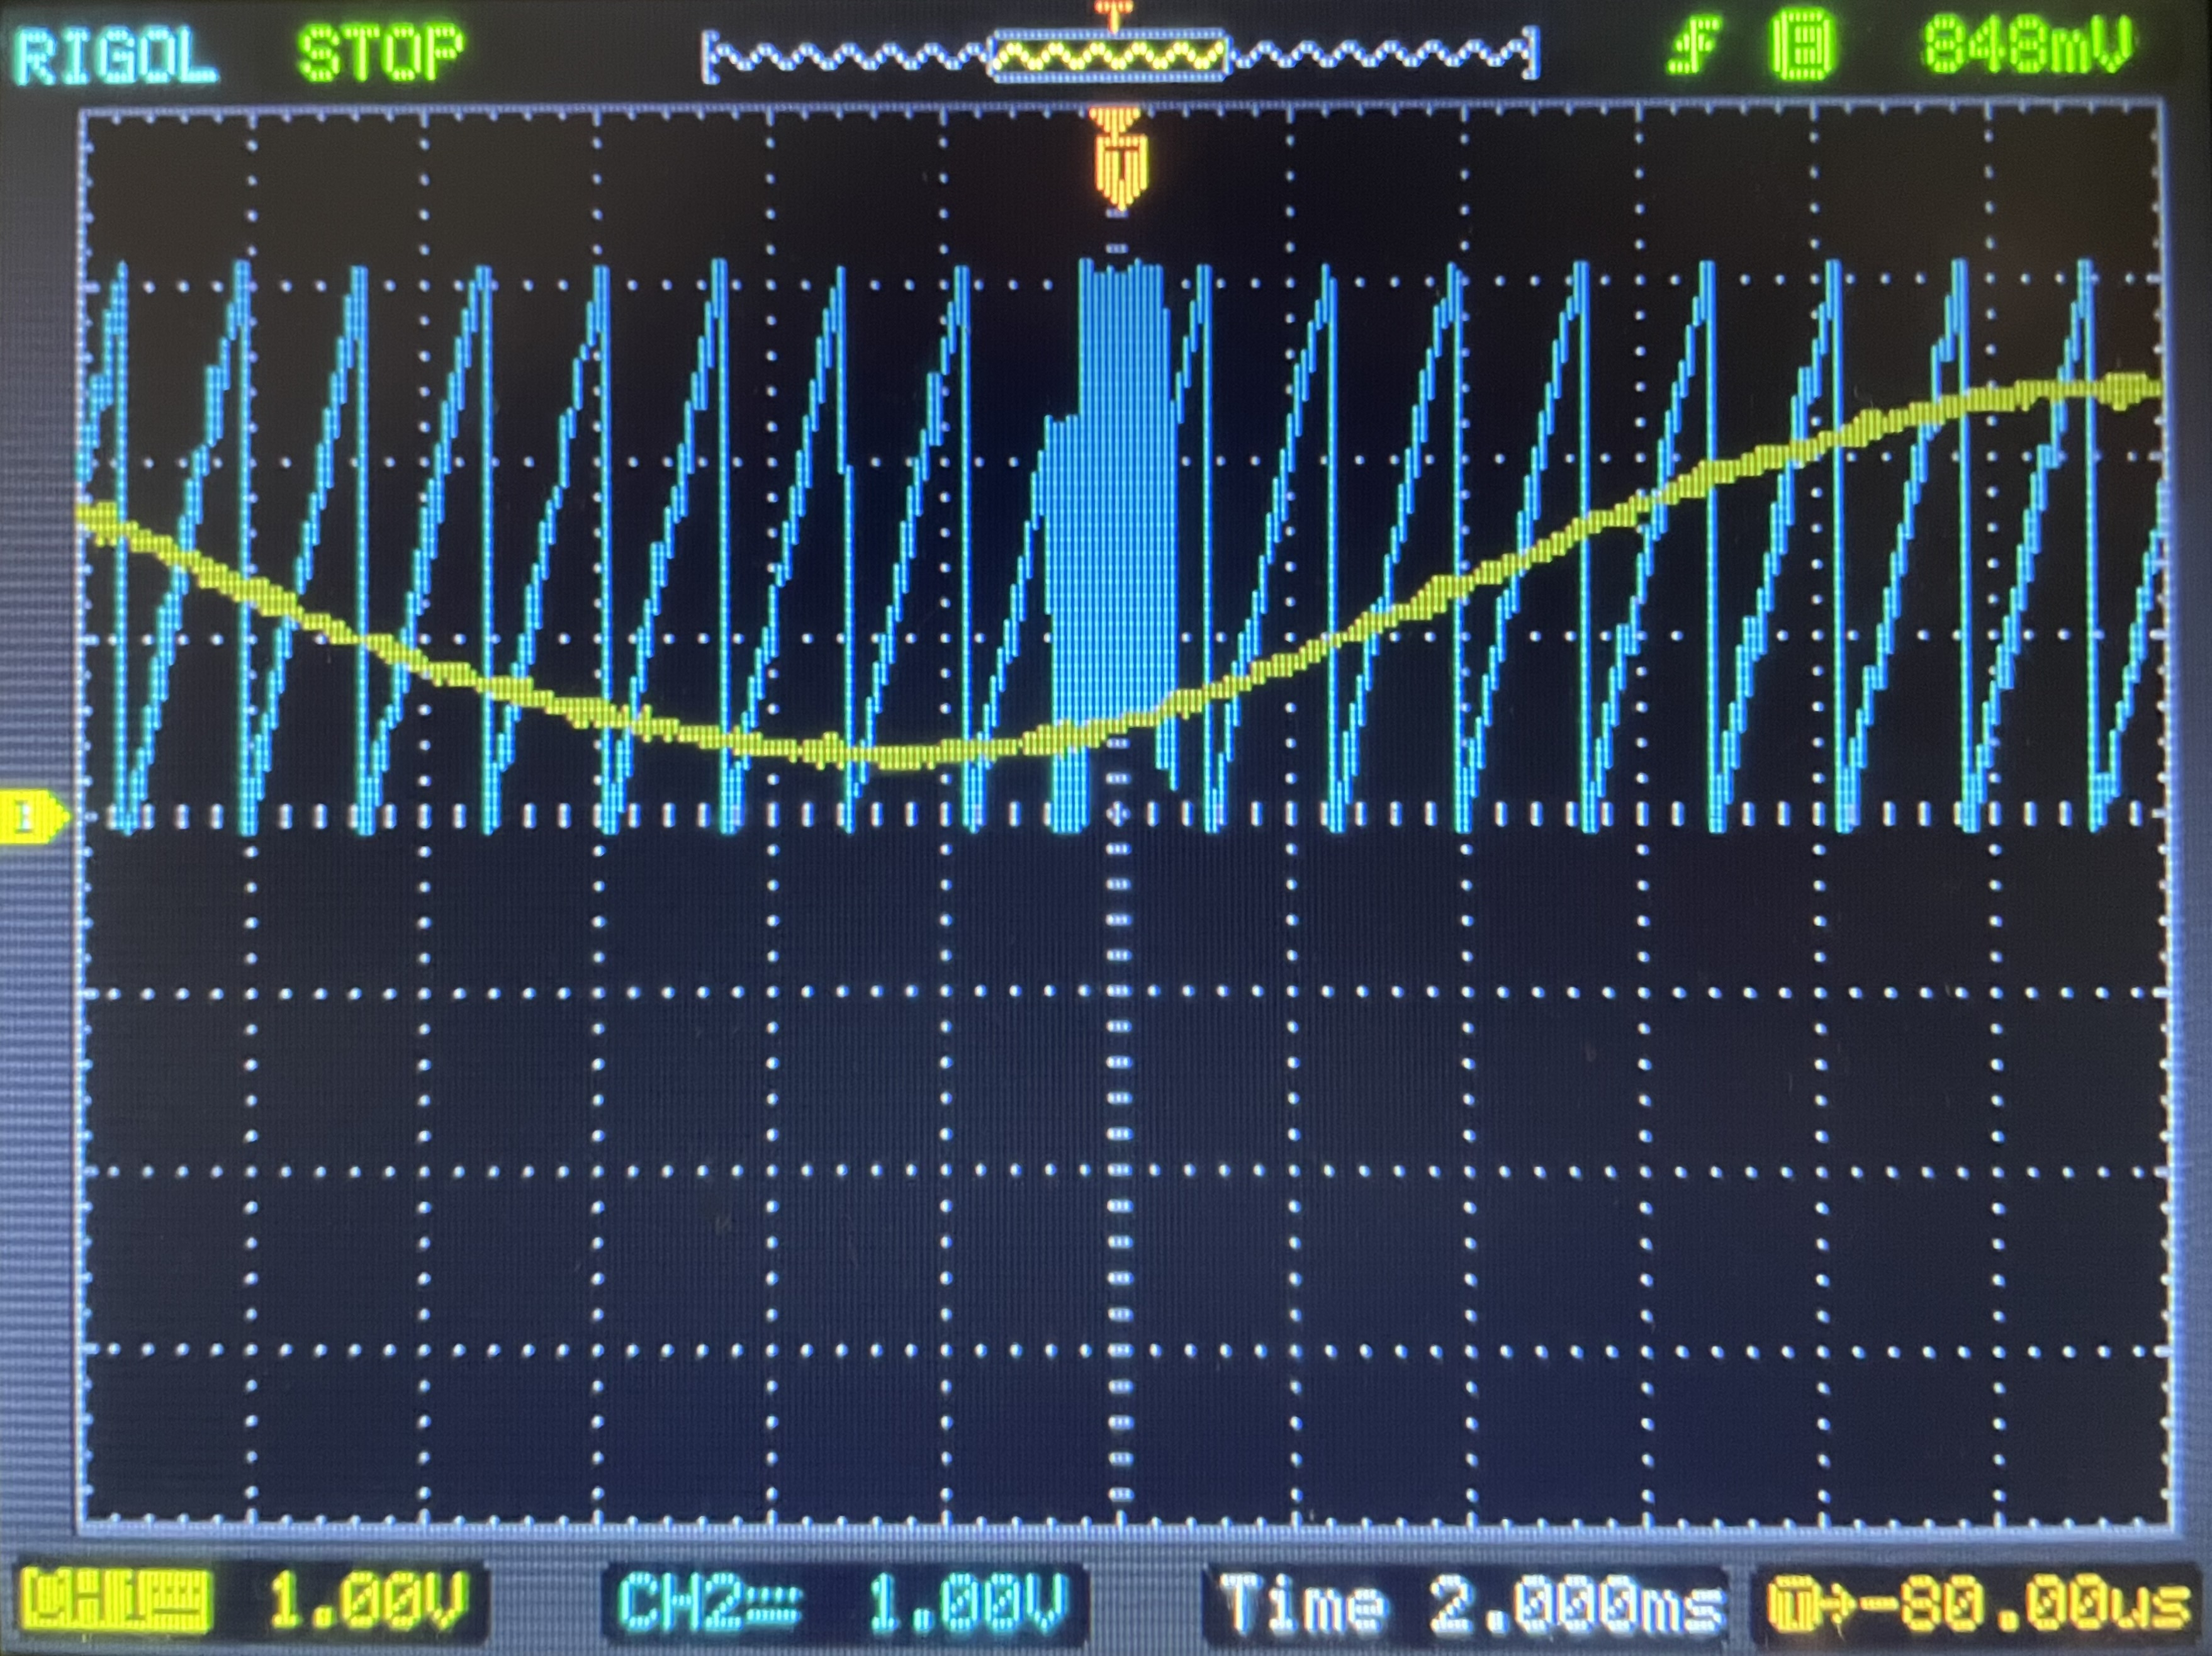
\includegraphics[width=0.95\linewidth]{position-calculated.jpeg}
    \caption[Calculated Beam Position Signal]{The calculated horizontal (blue) and vertical (yellow) position of the laser on the page, produced by the microcontroller in real time, used to determine whether or not to power the laser and illuminate this point on the screen, based on whether the desired image is bright in this position. The horizontal position is a simple periodic ramp, scanning linearly and resetting immediately to the start of its path as the beam encounters an edge of the polygon and the angle of incidence discontinuously changes, whereas the vertical position is a sine wave due the elliptical path of the beam form the rotating tilted mirror.}
    \label{fig:position-calculation-saw-sine}
\end{figure}



The position of the beam due to the tilted mirror is more complicated than the behavior of the scanning polygon mirror, and in fact due to the nonzero width of the ellipse contributes in part to the horizontal position. We use similar techniques as in the horizontal laser position calculation to compute the phase of the beam in its ellipse path, and take sine or cosine of this angular phase compute the x and y contributions of the ellipse to the beam position. To deal with the ellipse's eccentricity and rotation, we add two potentiometers the user can adjust to set these parameters, by simply tuning them until the image becomes coherent. To verify the microcontroller's computation of the beam path, we make it write the computed x and y position as PWM signals, put through an RC filter to convert to analog values read by the oscilloscope. The signals are shown in Figure~\ref{fig:position-calculation-saw-sine}. The vertical position is a sine wave, as expected due to the elliptical path, whereas the horizontal position is mainly a periodic ramp, as expected from the linear path which resets discontinuously from the polygon mirror. There is also a smaller cosine component to the ramp signal, not clearly visible in this signal due to the relative size of this cosine compared to the horizontal scanning of the polygon mirror (the ellipse was aligned so the narrow direction was mostly aligned across the direction of the horizontal scanning).

Driven at the prescribed maximum of 12 volts, the tilted mirror motor spun at around 5000 RPM, which with the $3000 RPM \times 12 sides = 36000$ scans per minute of the polygon mirror, would only allow for $36000/5000 \approx$ 7 lines per image, hardly enough to show anything useful. So we drive the tilt mirror motor at less than half power, slow enough to get more lines in an image, but barely above the minimum speed for human persistence of vision. To get additional lines in the image, we add a second projection laser, which due to slight differences in alignment traces a path slightly offset from the first. We add two potentiometers to adjust the resulting difference in x and y position between the two lasers' paths. These can easily be tuned when a double-image is seen to bring the images together into one coherent picture.



\section{Final Result}


Our final resulting laser projector could draw a convincing and recognizable simple image, demonstrated in Figure~\ref{fig:smiley} with a smiley face. Due to compromising between vertical resolution and drawing speed with our limited resources, a image or video camera wouldn't capture the whole image, although to the human eye it looked complete, so this figure is a composite of two frames form a video to show what the human eye sees with persistence of vision. 

\begin{figure*}[t]
    \centering
    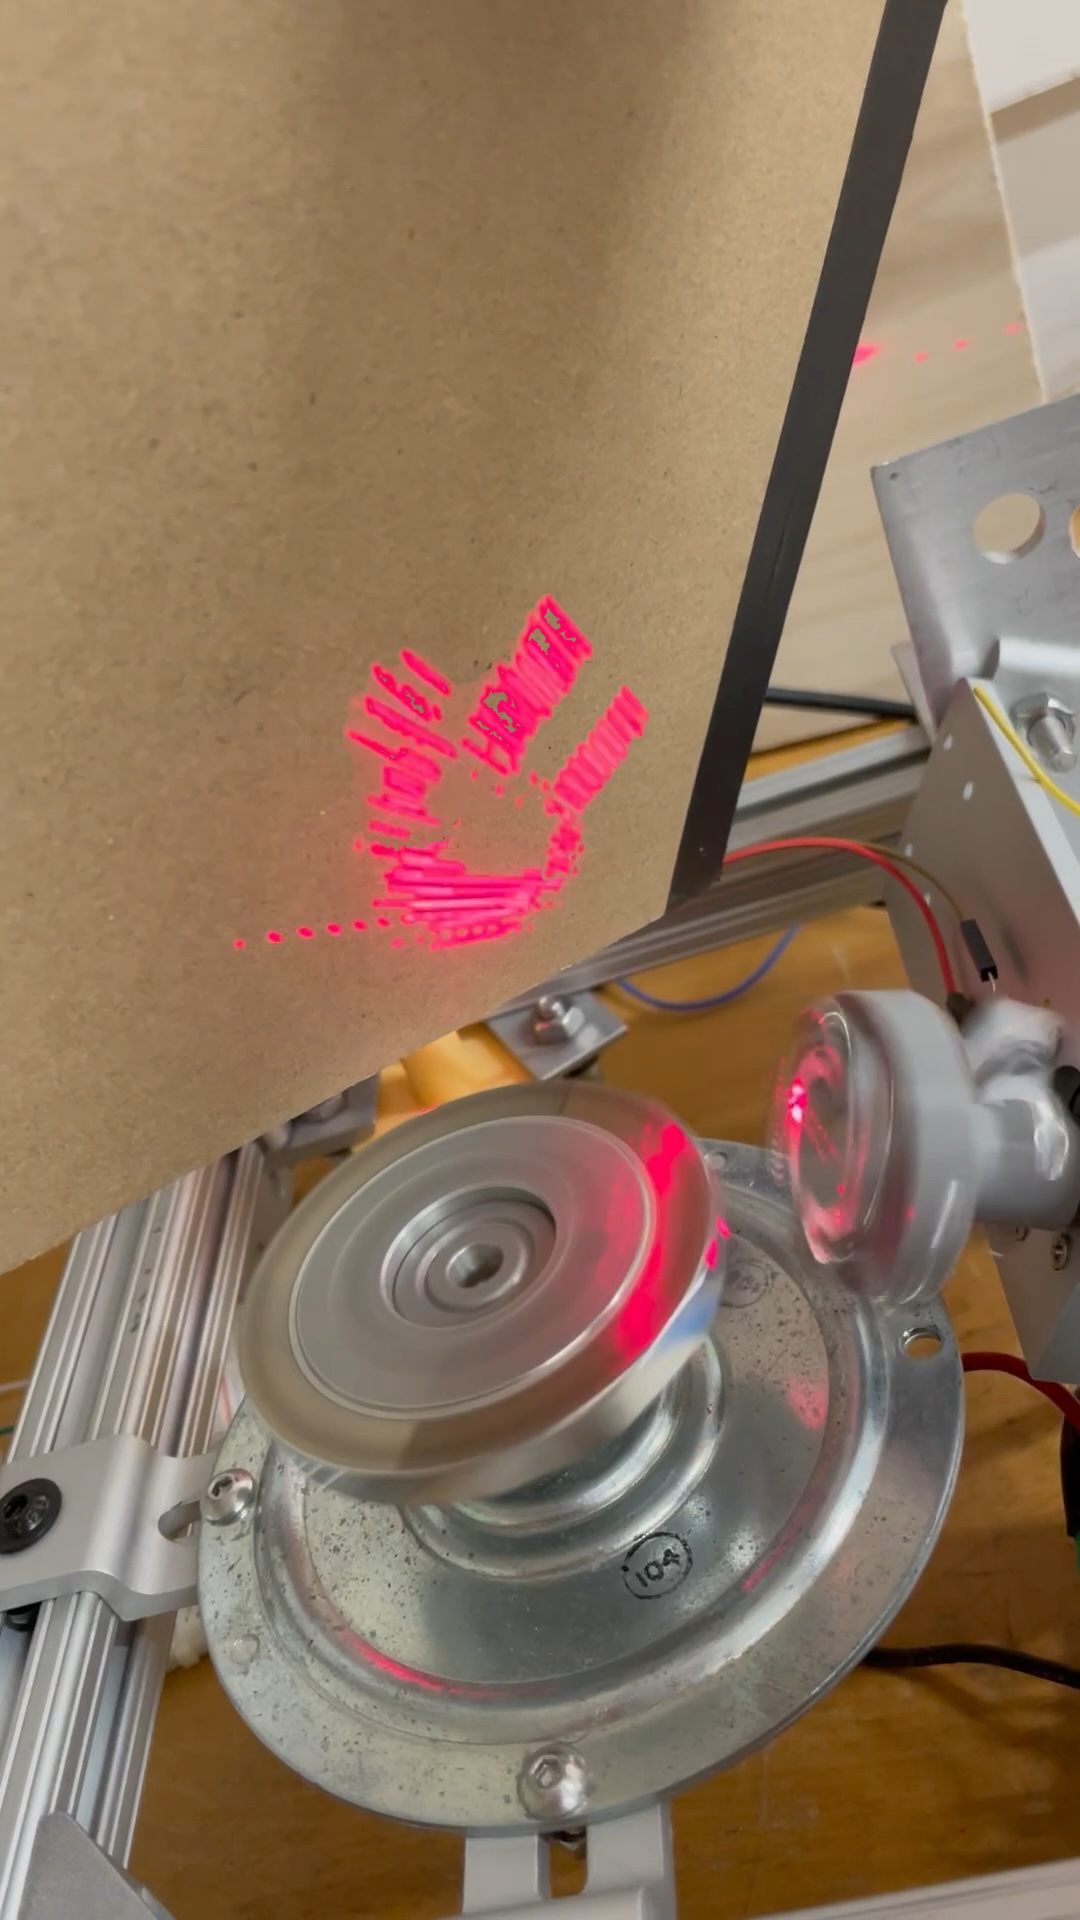
\includegraphics[width=0.80\linewidth]{smile-composite.jpeg}
    \caption[Final Demo: Drawing a Smile]{An image of a smiley face is drawn onto the screen by rapidly modulating the laser in time with the spinning mirrors with just the right timing to illuminate the right pixels.}
    \label{fig:smiley}
\end{figure*}

\section{Discussion}

The final product accomplishes the original goal of a laser projector, but is just barely within parameters. Moving mirrors at high speeds was a greater challenge than we initially estimated. Even with a polygon mirror not needing to fight inertia, our only enemy being dissipation,  at full power we could only just get the polygon spinning fast enough to draw enough lines within the persistence of vision timescale to show a convincing and recognizable image. At the down-adjusted speed of the tilted mirror, to allow for more lines at the cost of slower image rendering, the image could be seen in full although flickering and flashing was somewhat noticeable. Some minor timing signal detection or triggering issues make the apparatus occasionally misfire, sometimes drawing extraneous lines, such as the dotted line connecting to the smile shown in Figure~\ref{fig:smiley}. The 5mW red lasers, although bright when held still, become harder to see when rastering across an entire image quickly. The image couldn't be made out when projected directly on the wall as desired without turning the room lights off and potentially covering the windows if bright out. We attempted to upgrade to 10mW green lasers, but these came with some circuitry which had a finite time constant, enough to make modulating it at 100kHz not produce any output. At that point it was too late in the timeline to wait for new lasers to arrive, and none were available at a reasonable price to due shipping/tariff costs from China.

Still we are glad to have created a basic laser projector, requiring CAD modeling various parts, creating programs to compute moment of inertia tensors in CAD software, writing microcontroller code to analyze analog timing signals, compute beam paths, and modulate laser power all within a few microseconds, to engineer and construct the physical apparatus, and to debug and problem solve within constraints and unexpected hardware and software issues. We are especially glad of our creative low-cost solution to the problem normally solved by a high-speed galvanometer, with the rotation of a tilted mirror, and compensation for the  elliptical path this creates with software.

3D models created and code written for this project is available at \url{https://github.com/robertstrauss/laser-projector}.

\setlength{\parindent}{0cm}




\begin{thebibliography}{99}
\section*{Bibliography}


\bibitem{ben}
Ben Makes Everything (2024) \emph{DIY Laser Image Projector}, Youtube. \url{https://youtu.be/fEPicBSYeNQ?si=xe743wcq-36Dujjx}.

\bibitem{wyant}
Wyant College of Optical Sciences, "Persistence of Vision," The University of Arizona. \url{https://www.optics.arizona.edu/sites/default/files/2022-07/Persistence%20of%20Vision%20Pamphlet.pdf}

\end{thebibliography}

\setlength{\parindent}{0cm}

\end{document}

